% answers.tex —— 1992 年·全国卷·理科 · 参考答案与详细解析片段
% 由 tools/generate_projects.py 依来源总账自 1992/1992_数学真题_全国理_试题.md + 1992/1992_数学真题_全国理_解析正文.md + 1992/1992_数学真题_全国理_答案要点.md 生成，勿手改（改源 MD 后重跑）


\begin{gktip}
固定源 PDF 不附答案。以下解析由编者依据固定题面独立推导，非官方解析；第 16 题源内函数式缺损（\(e^x-e^x\)），按通常命题意图给出条件结论并注明。
\end{gktip}

\begin{answer}
\gksolhead{1}{}

\textbf{题目}：

\(\dfrac{\log_8 9}{\log_2 3}\) 的值是（　）

(A) \(\dfrac{2}{3}\)　(B) \(1\)　(C) \(\dfrac{3}{2}\)　(D) \(2\)

\Needspace{4\baselineskip}
\textbf{解析}

\Needspace{5\baselineskip}
由换底公式，
\nopagebreak[4]
\[
\frac{\log_8 9}{\log_2 3}
=\frac{\log_2 9/\log_2 8}{\log_2 3}
=\frac{2\log_2 3/3}{\log_2 3}
=\frac23.
\]

\gkanswer{答案：A}

\end{answer}
\begin{answer}
\gksolhead{2}{}

\textbf{题目}：

如果函数 \(y=\sin(\omega x)\cos(\omega x)\) 的最小正周期是 \(4\pi\)，那么常数 \(\omega\) 为（　）

(A) \(4\)　(B) \(2\)　(C) \(\dfrac{1}{2}\)　(D) \(\dfrac{1}{4}\)

\Needspace{4\baselineskip}
\textbf{解析}

\Needspace{5\baselineskip}
\(y=\sin(\omega x)\cos(\omega x)=\dfrac12\sin 2\omega x\)，最小正周期
\nopagebreak[4]
\[
T=\frac{2\pi}{2|\omega|}=\frac{\pi}{|\omega|}=4\pi,
\]
故 \(|\omega|=\dfrac14\)，取正值得 \(\omega=\dfrac14\)。

\gkanswer{答案：D}

\end{answer}
\begin{answer}
\gksolhead{3}{}

\textbf{题目}：

极坐标方程分别是 \(\rho=\cos\theta\) 和 \(\rho=\sin\theta\) 的两个圆的圆心距是（　）

(A) \(2\)　(B) \(\sqrt{2}\)　(C) \(1\)　(D) \(\dfrac{\sqrt{2}}{2}\)

\Needspace{4\baselineskip}
\textbf{解析}

\Needspace{5\baselineskip}
由 \(\rho=\cos\theta\) 得 \(\rho^2=\rho\cos\theta\)，即 \(x^2+y^2=x\)，圆心 \(\left(\dfrac12,0\right)\)；由 \(\rho=\sin\theta\) 得 \(x^2+y^2=y\)，圆心 \(\left(0,\dfrac12\right)\)。圆心距
\nopagebreak[4]
\[
\sqrt{\left(\frac12\right)^2+\left(\frac12\right)^2}=\frac{\sqrt2}{2}.
\]

\gkanswer{答案：D}

\end{answer}
\begin{answer}
\gksolhead{4}{}

\textbf{题目}：

方程 \(\sin 4x\cos 5x=-\cos 4x\sin 5x\) 的一个解是（　）

(A) \(10^{\circ}\)　(B) \(20^{\circ}\)　(C) \(50^{\circ}\)　(D) \(70^{\circ}\)

\Needspace{4\baselineskip}
\textbf{解析}

移项得 \(\sin4x\cos5x+\cos4x\sin5x=0\)，即 \(\sin9x=0\)，故 \(x=\dfrac{k\pi}{9}=20^\circ k\ (k\in\mathbb Z)\)。取 \(k=1\) 得 \(20^\circ\)，在所给选项中。

\gkanswer{答案：B}

\end{answer}
\begin{answer}
\gksolhead{5}{}

\textbf{题目}：

已知轴截面是正方形的圆柱的高与球的直径相等，则圆柱的全面积与球的表面积的比是（　）

(A) \(6:5\)　(B) \(5:4\)　(C) \(4:3\)　(D) \(3:2\)

\Needspace{4\baselineskip}
\textbf{解析}

\Needspace{5\baselineskip}
设圆柱底面半径为 \(r\)，高为 \(h\)。轴截面为正方形，故 \(h=2r\)；又高与球的直径相等，故球半径 \(R=r\)。圆柱全面积
\nopagebreak[4]
\[
S_{\text{柱}}=2\pi r^2+2\pi rh=2\pi r^2+4\pi r^2=6\pi r^2,
\]
球表面积 \(S_{\text{球}}=4\pi R^2=4\pi r^2\)，比值 \(6:4=3:2\)。

\gkanswer{答案：D}

\end{answer}
\begin{answer}
\gksolhead{6}{}

\textbf{题目}：

如图，图中曲线是幂函数 \(y=x^{n}\) 在第一象限的图象。已知 \(n\) 取 \(\pm 2\)，\(\pm\dfrac{1}{2}\) 四个值，则相应于曲线 \(C_1\)、\(C_2\)、\(C_3\)、\(C_4\) 的 \(n\) 依次为（　）
\nopagebreak[4]
\begin{center}% f1992nl_q06_power_curves.tex — 1992 年·全国卷·理科 第 6 题（幂函数四曲线）
%
% 【来源】`.work/phase4-b15/source/1992全国理.pdf`（SHA-256 aa3c0a314b5ea0bf990cbc7d768575e3b3931da6ddbfb6c727681a516a7eb7aa），
%   第 1 页（印刷页 42）；内容流逐路径实测见 `.work/phase4-b15/transcripts/science-figures.md`。
%
% 【坐标口径】源 PDF 用户空间（原点左下、y 向上）。本图本地坐标
%   (x, y) = (x_page − 184.0000, y_page − 311.0000)，1 单位 = 1 TeX pt。
%   路径坐标逐点照录内容流（含三次贝塞尔控制点）。
%
% 元素计数：8 条路径（两轴＋两箭头＋四曲线）＋8 个标签
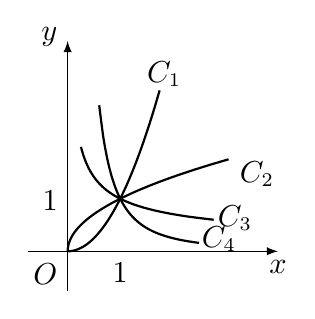
\begin{tikzpicture}[x=1pt, y=1pt,
    every node/.style={inner sep=0pt, font=\fontsize{10.5pt}{12.6pt}\selectfont}]
  \draw[line width=0.398pt] (4.1758,5.6150)   -- (90.8028,5.6150);
  \fill[line width=1.0pt] (94.3892,5.6150)   .. controls (93.3262,5.8140) and (91.5992,6.4120) .. (90.4042,7.1090)   -- (90.4042,4.1210)   .. controls (91.5992,4.8180) and (93.3262,5.4160) .. (94.3892,5.6150);
  \draw[line width=0.398pt] (18.4200,-8.6292)   -- (18.4200,77.9978);
  \fill[line width=1.0pt] (18.4200,81.5842)   .. controls (18.2210,80.5212) and (17.6230,78.7942) .. (16.9260,77.5992)   -- (19.9140,77.5992)   .. controls (19.2170,78.7942) and (18.6190,80.5212) .. (18.4200,81.5842);
  \draw[line width=0.797pt] (18.4200,5.6150)   .. controls (18.4200,5.6150) and (19.4200,5.6600) .. (19.8050,5.7160)   .. controls (20.1890,5.7720) and (20.8050,5.9070) .. (21.1890,6.0190)   .. controls (21.5740,6.1310) and (22.1900,6.3550) .. (22.5740,6.5240)   .. controls (22.9580,6.6920) and (23.5740,7.0060) .. (23.9590,7.2300)   .. controls (24.3430,7.4540) and (24.9590,7.8580) .. (25.3430,8.1390)   .. controls (25.7280,8.4190) and (26.3440,8.9130) .. (26.7280,9.2490)   .. controls (27.1120,9.5850) and (27.7280,10.1690) .. (28.1130,10.5620)   .. controls (28.4970,10.9540) and (29.1130,11.6280) .. (29.4970,12.0760)   .. controls (29.8820,12.5240) and (30.4980,13.2880) .. (30.8820,13.7920)   .. controls (31.2660,14.2960) and (31.8820,15.1500) .. (32.2670,15.7100)   .. controls (32.6510,16.2700) and (33.2670,17.2140) .. (33.6510,17.8300)   .. controls (34.0360,18.4460) and (34.6520,19.4800) .. (35.0360,20.1520)   .. controls (35.4200,20.8240) and (36.0360,21.9470) .. (36.4210,22.6750)   .. controls (36.8050,23.4040) and (37.4210,24.6170) .. (37.8050,25.4010)   .. controls (38.1890,26.1860) and (38.8060,27.4890) .. (39.1900,28.3290)   .. controls (39.5740,29.1690) and (40.1900,30.5620) .. (40.5750,31.4580)   .. controls (40.9590,32.3550) and (41.5750,33.8370) .. (41.9590,34.7900)   .. controls (42.3430,35.7420) and (42.9600,37.3140) .. (43.3440,38.3230)   .. controls (43.7280,39.3310) and (44.3440,40.9940) .. (44.7290,42.0580)   .. controls (45.1130,43.1230) and (45.7290,44.8750) .. (46.1130,45.9950)   .. controls (46.4970,47.1160) and (47.1140,48.9580) .. (47.4980,50.1340)   .. controls (47.8820,51.3110) and (48.4980,53.2430) .. (48.8830,54.4750)   .. controls (49.2670,55.7080) and (49.8830,57.7290) .. (50.2670,59.0180)   .. controls (50.6510,60.3060) and (51.6520,63.7630) .. (51.6520,63.7630);
  \draw[line width=0.797pt] (18.4200,5.6150)   .. controls (18.4200,5.6150) and (18.4650,6.6150) .. (18.5210,7.0000)   .. controls (18.5770,7.3840) and (18.7120,8.0000) .. (18.8240,8.3840)   .. controls (18.9360,8.7690) and (19.1600,9.3850) .. (19.3290,9.7690)   .. controls (19.4970,10.1530) and (19.8110,10.7690) .. (20.0350,11.1540)   .. controls (20.2590,11.5380) and (20.6630,12.1540) .. (20.9440,12.5380)   .. controls (21.2240,12.9230) and (21.7180,13.5390) .. (22.0540,13.9230)   .. controls (22.3900,14.3070) and (22.9740,14.9230) .. (23.3670,15.3080)   .. controls (23.7590,15.6920) and (24.4330,16.3080) .. (24.8810,16.6920)   .. controls (25.3290,17.0770) and (26.0930,17.6930) .. (26.5970,18.0770)   .. controls (27.1010,18.4610) and (27.9550,19.0770) .. (28.5150,19.4620)   .. controls (29.0750,19.8460) and (30.0190,20.4620) .. (30.6350,20.8460)   .. controls (31.2510,21.2310) and (32.2850,21.8470) .. (32.9570,22.2310)   .. controls (33.6290,22.6150) and (34.7520,23.2310) .. (35.4800,23.6160)   .. controls (36.2090,24.0000) and (37.4220,24.6160) .. (38.2060,25.0000)   .. controls (38.9910,25.3840) and (40.2940,26.0010) .. (41.1340,26.3850)   .. controls (41.9740,26.7690) and (43.3670,27.3850) .. (44.2630,27.7700)   .. controls (45.1600,28.1540) and (46.6420,28.7700) .. (47.5950,29.1540)   .. controls (48.5470,29.5380) and (50.1190,30.1550) .. (51.1280,30.5390)   .. controls (52.1360,30.9230) and (53.7990,31.5390) .. (54.8630,31.9240)   .. controls (55.9280,32.3080) and (57.6800,32.9240) .. (58.8000,33.3080)   .. controls (59.9210,33.6920) and (61.7630,34.3090) .. (62.9390,34.6930)   .. controls (64.1160,35.0770) and (66.0480,35.6930) .. (67.2800,36.0780)   .. controls (68.5130,36.4620) and (70.5340,37.0780) .. (71.8230,37.4620)   .. controls (73.1110,37.8460) and (76.5680,38.8470) .. (76.5680,38.8470);
  \draw[line width=0.797pt] (29.8155,58.3765)   .. controls (29.8155,58.3765) and (30.9015,49.5285) .. (31.3185,46.7905)   .. controls (31.7365,44.0515) and (32.4055,40.5955) .. (32.8225,38.6395)   .. controls (33.2395,36.6845) and (33.9085,34.1395) .. (34.3255,32.6925)   .. controls (34.7435,31.2465) and (35.4125,29.3175) .. (35.8295,28.2175)   .. controls (36.2465,27.1175) and (36.9155,25.6175) .. (37.3325,24.7625)   .. controls (37.7505,23.9085) and (38.4195,22.7335) .. (38.8365,22.0565)   .. controls (39.2535,21.3785) and (39.9225,20.4265) .. (40.3395,19.8785)   .. controls (40.7575,19.3305) and (41.4265,18.5545) .. (41.8435,18.1065)   .. controls (42.2605,17.6575) and (42.9295,17.0175) .. (43.3465,16.6455)   .. controls (43.7645,16.2725) and (44.4335,15.7355) .. (44.8505,15.4245)   .. controls (45.2675,15.1125) and (45.9365,14.6625) .. (46.3535,14.3985)   .. controls (46.7705,14.1345) and (47.4405,13.7475) .. (47.8575,13.5225)   .. controls (48.2745,13.2965) and (48.9435,12.9675) .. (49.3605,12.7735)   .. controls (49.7775,12.5795) and (50.4475,12.2925) .. (50.8645,12.1245)   .. controls (51.2815,11.9555) and (51.9505,11.7075) .. (52.3675,11.5605)   .. controls (52.7845,11.4145) and (53.4535,11.1965) .. (53.8715,11.0675)   .. controls (54.2885,10.9395) and (54.9575,10.7465) .. (55.3745,10.6325)   .. controls (55.7915,10.5195) and (56.4605,10.3485) .. (56.8785,10.2485)   .. controls (57.2955,10.1475) and (57.9645,9.9955) .. (58.3815,9.9055)   .. controls (58.7985,9.8155) and (59.4675,9.6805) .. (59.8855,9.6005)   .. controls (60.3025,9.5205) and (60.9715,9.3995) .. (61.3885,9.3265)   .. controls (61.8055,9.2545) and (62.4745,9.1445) .. (62.8925,9.0795)   .. controls (63.3095,9.0135) and (63.9785,8.9145) .. (64.3955,8.8555)   .. controls (64.8125,8.7965) and (65.8985,8.6545) .. (65.8985,8.6545);
  \draw[line width=0.797pt] (71.1815,17.0105)   .. controls (71.1815,17.0105) and (64.4925,17.8035) .. (62.3185,18.1085)   .. controls (60.1445,18.4125) and (57.1965,18.9015) .. (55.5115,19.2055)   .. controls (53.8255,19.5105) and (51.5035,19.9995) .. (50.1705,20.3035)   .. controls (48.8385,20.6085) and (46.9795,21.0965) .. (45.9075,21.4015)   .. controls (44.8365,21.7065) and (43.3245,22.1945) .. (42.4495,22.4995)   .. controls (41.5745,22.8035) and (40.3255,23.2925) .. (39.6035,23.5975)   .. controls (38.8815,23.9015) and (37.8505,24.3905) .. (37.2465,24.6945)   .. controls (36.6435,24.9995) and (35.7635,25.4875) .. (35.2525,25.7925)   .. controls (34.7405,26.0975) and (33.9945,26.5855) .. (33.5585,26.8905)   .. controls (33.1225,27.1945) and (32.4845,27.6835) .. (32.1095,27.9885)   .. controls (31.7345,28.2925) and (31.1835,28.7815) .. (30.8595,29.0855)   .. controls (30.5345,29.3905) and (30.0565,29.8785) .. (29.7735,30.1835)   .. controls (29.4905,30.4885) and (29.0695,30.9765) .. (28.8215,31.2815)   .. controls (28.5735,31.5865) and (28.2055,32.0745) .. (27.9875,32.3795)   .. controls (27.7695,32.6835) and (27.4415,33.1725) .. (27.2475,33.4765)   .. controls (27.0535,33.7815) and (26.7635,34.2705) .. (26.5915,34.5745)   .. controls (26.4185,34.8795) and (26.1585,35.3675) .. (26.0045,35.6725)   .. controls (25.8505,35.9775) and (25.6195,36.4655) .. (25.4805,36.7705)   .. controls (25.3425,37.0745) and (25.1325,37.5635) .. (25.0075,37.8675)   .. controls (24.8825,38.1725) and (24.6925,38.6615) .. (24.5805,38.9655)   .. controls (24.4675,39.2705) and (24.2975,39.7585) .. (24.1945,40.0635)   .. controls (24.0925,40.3685) and (23.9355,40.8565) .. (23.8425,41.1615)   .. controls (23.7485,41.4655) and (23.6065,41.9545) .. (23.5215,42.2585)   .. controls (23.4375,42.5635) and (23.2305,43.3565) .. (23.2305,43.3565);

  \node[anchor=center] at (11.800,83.000) {$y$};  % 源中心 (195.80,394.00)
  \node[anchor=center] at (94.400,0.000) {$x$};  % 源中心 (278.40,311.00)
  \node[anchor=center] at (10.400,-2.600) {$O$};  % 源中心 (194.40,308.40)
  \node[anchor=center] at (37.400,-2.200) {$1$};  % 源中心 (221.40,308.80)
  \node[anchor=center] at (12.100,23.800) {$1$};  % 源中心 (196.10,334.80)
  \node[anchor=center] at (53.300,69.600) {$C_1$};  % 源中心 (237.30,380.60)
  \node[anchor=center] at (86.800,33.500) {$C_2$};  % 源中心 (270.80,344.50)
  \node[anchor=center] at (78.900,17.600) {$C_3$};  % 源中心 (262.90,328.60)
  \node[anchor=center] at (73.100,10.000) {$C_4$};  % 源中心 (257.10,321.00)

\end{tikzpicture}
%
% 【自验结果】
%   探针：见 .work/phase4-b15/probe 的 verify_paths.py / check600_b15.py。
\end{center}
\nopagebreak[4]
(A) \(-2\)，\(-\dfrac{1}{2}\)，\(\dfrac{1}{2}\)，\(2\)　(B) \(2\)，\(\dfrac{1}{2}\)，\(-\dfrac{1}{2}\)，\(-2\)　(C) \(-\dfrac{1}{2}\)，\(-2\)，\(2\)，\(\dfrac{1}{2}\)　(D) \(2\)，\(\dfrac{1}{2}\)，\(-2\)，\(-\dfrac{1}{2}\)

\Needspace{4\baselineskip}
\textbf{解析}

四条曲线都过 \((1,1)\)。当 \(x>1\) 时 \(x^{2}>x^{1/2}>1>x^{-1/2}>x^{-2}\)，与图中自上而下的 \(C_1,C_2,C_3,C_4\) 对应，故 \(n\) 依次为 \(2,\dfrac12,-\dfrac12,-2\)。

\gkanswer{答案：B}

\end{answer}
\begin{answer}
\gksolhead{7}{}

\textbf{题目}：

若 \(\log_a 2<\log_b 2<0\)，则（　）

(A) \(0<a<b<1\)　(B) \(0<b<a<1\)　(C) \(a>b>1\)　(D) \(b>a>1\)

\Needspace{4\baselineskip}
\textbf{解析}

\Needspace{5\baselineskip}
若 \(a>1\)，则 \(\log_a2>0\)，与题设矛盾，故 \(0<a<1\)；同理 \(0<b<1\)。此时
\nopagebreak[4]
\[
\log_a2=\frac{1}{\log_2 a},\qquad \log_b2=\frac{1}{\log_2 b},
\]
且 \(\log_2 a<0,\ \log_2 b<0\)。由 \(\dfrac{1}{\log_2 a}<\dfrac{1}{\log_2 b}<0\)，两边乘正数 \(\log_2 a\cdot\log_2 b\) 得 \(\log_2 b<\log_2 a\)，即 \(b<a\)。故 \(0<b<a<1\)。

\gkanswer{答案：B}

\end{answer}
\begin{answer}
\gksolhead{8}{}

\textbf{题目}：

直线 \(\begin{cases}x=t\cdot\sin 20^{\circ}+3,\\ y=-t\cdot\cos 20^{\circ},\end{cases}\)（\(t\) 为参数）的倾斜角是（　）

(A) \(20^{\circ}\)　(B) \(70^{\circ}\)　(C) \(110^{\circ}\)　(D) \(160^{\circ}\)

\Needspace{4\baselineskip}
\textbf{解析}

\Needspace{5\baselineskip}
方向向量为 \((\sin20^\circ,-\cos20^\circ)=(\cos70^\circ,-\sin70^\circ)\)，斜率
\nopagebreak[4]
\[
k=-\cot20^\circ=\tan110^\circ,
\]
故倾斜角为 \(110^\circ\)（取 \([0^\circ,180^\circ)\)）。

\gkanswer{答案：C}

\end{answer}
\begin{answer}
\gksolhead{9}{}

\textbf{题目}：

在四棱锥的四个侧面中，直角三角形最多可有（　）

(A) \(1\) 个　(B) \(2\) 个　(C) \(3\) 个　(D) \(4\) 个

\Needspace{4\baselineskip}
\textbf{解析}

取四棱锥 \(S\text{-}ABCD\)，使 \(SA\perp\) 底面，底面 \(ABCD\) 为矩形。则 \(\angle SAB=\angle SAD=90^\circ\)；又 \(BC\perp AB\)，\(BC\perp SA\)，故 \(BC\perp\) 平面 \(SAB\)，从而 \(BC\perp SB\)，\(\angle SBC=90^\circ\)；同理 \(\angle SDC=90^\circ\)。四个侧面全为直角三角形，而侧面总数只有 4 个，故最多 4 个。

\gkanswer{答案：D}

\end{answer}
\begin{answer}
\gksolhead{10}{}

\textbf{题目}：

圆心在抛物线 \(y^{2}=2x\) 上，且与 \(x\) 轴和该抛物线的准线都相切的一个圆的方程是（　）

(A) \(x^{2}+y^{2}-x-2y-\dfrac{1}{4}=0\)　(B) \(x^{2}+y^{2}+x-2y+1=0\)　(C) \(x^{2}+y^{2}-x-2y+1=0\)　(D) \(x^{2}+y^{2}-x-2y+\dfrac{1}{4}=0\)

\Needspace{4\baselineskip}
\textbf{解析}

\Needspace{5\baselineskip}
抛物线 \(y^2=2x\) 的准线为 \(x=-\dfrac12\)。设圆心 \((a,b)\)，则 \(b^2=2a\)；与 \(x\) 轴相切得半径 \(r=|b|\)，与准线相切得 \(r=a+\dfrac12\)。于是
\nopagebreak[4]
\[
|b|=\frac{b^2}{2}+\frac12.
\]
\Needspace{5\baselineskip}
令 \(u=|b|\ge0\)，得 \(u^2-2u+1=0\)，即 \(u=1\)。故 \(a=\dfrac12\)，\(b=\pm1\)，\(r=1\)。取 \(b=1\) 得
\nopagebreak[4]
\[
\left(x-\frac12\right)^2+(y-1)^2=1,
\]
即 \(x^2+y^2-x-2y+\dfrac14=0\)。（另一解圆心 \(\left(\dfrac12,-1\right)\) 不在选项中。）

\gkanswer{答案：D}

\end{answer}
\begin{answer}
\gksolhead{11}{}

\textbf{题目}：

在 \((x^{2}+3x+2)^{5}\) 的展开式中 \(x\) 的系数为（　）

(A) \(160\)　(B) \(240\)　(C) \(360\)　(D) \(800\)

\Needspace{4\baselineskip}
\textbf{解析}

\Needspace{5\baselineskip}
\((x^2+3x+2)^5\) 中产生 \(x\) 一次项的只能是「恰有一个括号取 \(3x\)、其余四个括号取 \(2\)」，故系数为
\nopagebreak[4]
\[
\binom51\cdot3\cdot2^4=5\cdot3\cdot16=240.
\]

\gkanswer{答案：B}

\end{answer}
\begin{answer}
\gksolhead{12}{}

\textbf{题目}：

若 \(0<a<1\)，在 \([0,2\pi]\) 上满足 \(\sin x\geqslant a\) 的 \(x\) 的范围是（　）

(A) \([0,\arcsin a]\)　(B) \([\arcsin a,\ \pi-\arcsin a]\)　(C) \([\pi-\arcsin a,\ \pi]\)　(D) \(\left[\arcsin a,\ \dfrac{\pi}{2}+\arcsin a\right]\)

\Needspace{4\baselineskip}
\textbf{解析}

\Needspace{5\baselineskip}
\(0<a<1\) 时 \(\arcsin a\in\left(0,\dfrac{\pi}{2}\right)\)。在 \([0,2\pi]\) 上，\(\sin x\geqslant a\) 的两端点解为 \(x=\arcsin a\) 与 \(x=\pi-\arcsin a\)，其间满足不等式，故范围为
\nopagebreak[4]
\[
[\arcsin a,\ \pi-\arcsin a].
\]

\gkanswer{答案：B}

\end{answer}
\begin{answer}
\gksolhead{13}{}

\textbf{题目}：

已知直线 \(l_1\) 和 \(l_2\) 夹角的平分线为 \(y=x\)，如果 \(l_1\) 的方程是 \(ax+by+c=0\)（\(ab>0\)），那么 \(l_2\) 的方程是（　）

(A) \(bx+ay+c=0\)　(B) \(ax-by+c=0\)　(C) \(bx+ay-c=0\)　(D) \(bx-ay+c=0\)

\Needspace{4\baselineskip}
\textbf{解析}

关于 \(y=x\) 的对称变换即交换 \(x,y\)。\(l_1:ax+by+c=0\) 的对称直线为 \(ay+bx+c=0\)，即 \(bx+ay+c=0\)。由于 \(y=x\) 是 \(l_1,l_2\) 夹角的平分线且 \(l_2\neq l_1\)，故 \(l_2\) 即为该对称直线。

\gkanswer{答案：A}

\end{answer}
\begin{answer}
\gksolhead{14}{}

\textbf{题目}：

如图，在棱长为 \(1\) 的正方体 \(ABCD-A_1B_1C_1D_1\) 中，\(M\) 和 \(N\) 分别为 \(A_1B_1\) 和 \(BB_1\) 的中点，那么直线 \(AM\) 与 \(CN\) 所成角的余弦值是（　）
\nopagebreak[4]
\begin{center}% f1992nl_q14_cube.tex — 1992 年·全国卷·理科 第 14 题（正方体与中点）
%
% 【来源】`.work/phase4-b15/source/1992全国理.pdf`（SHA-256 aa3c0a314b5ea0bf990cbc7d768575e3b3931da6ddbfb6c727681a516a7eb7aa），
%   第 1 页（印刷页 42）；内容流逐路径实测见 `.work/phase4-b15/transcripts/science-figures.md`。
%
% 【坐标口径】源 PDF 用户空间（原点左下、y 向上）。本图本地坐标
%   (x, y) = (x_page − 553.0000, y_page − 375.0000)，1 单位 = 1 TeX pt。
%   路径坐标逐点照录内容流（含三次贝塞尔控制点）。
%
% 元素计数：2 组路径（9 实＋3 虚＋AM/CN）＋10 个标签
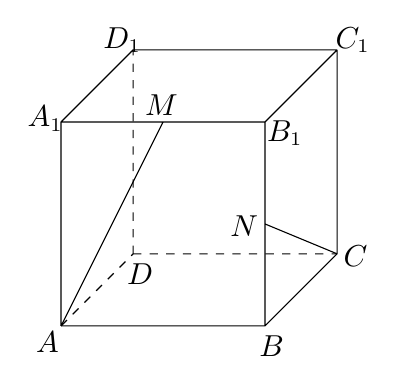
\begin{tikzpicture}[x=1pt, y=1pt,
    every node/.style={inner sep=0pt, font=\fontsize{10.5pt}{12.6pt}\selectfont}]
  \draw[line width=0.398pt] (5.6070,13.0830)   -- (79.3100,13.0830)   (79.3100,13.0830)   -- (105.3650,39.1370)   (79.3100,49.9350)   -- (105.3650,39.1370)   (5.6070,13.0830)   -- (42.4590,86.7860)   (5.6070,86.7860)   -- (79.3100,86.7860)   (79.3100,13.0830)   -- (79.3100,86.7860)   (5.6070,13.0830)   -- (5.6070,86.7860)   (105.3650,112.8410)   -- (79.3100,86.7860)   (105.3650,112.8410)   -- (31.6610,112.8410)   (5.6070,86.7860)   -- (31.6610,112.8410)   (5.6070,86.7860)   -- (5.6070,13.0830)   (79.3100,86.7860)   -- (79.3100,13.0830)   (105.3650,112.8410)   -- (105.3650,39.1370);
  \draw[line width=0.398pt, dash pattern=on 2.989pt off 2.989pt, dash phase=0.0pt] (5.6070,13.0830)   -- (31.6610,39.1370)   (31.6610,39.1370)   -- (105.3650,39.1370)   (31.6610,39.1370)   -- (31.6610,112.8410);

  \node[anchor=center] at (-0.100,88.000) {$A_1$};  % 源中心 (552.90,463.00)
  \node[anchor=center] at (86.500,82.700) {$B_1$};  % 源中心 (639.50,457.70)
  \node[anchor=center] at (111.000,116.300) {$C_1$};  % 源中心 (664.00,491.30)
  \node[anchor=center] at (27.700,116.300) {$D_1$};  % 源中心 (580.70,491.30)
  \node[anchor=center] at (0.700,7.200) {$A$};  % 源中心 (553.70,382.20)
  \node[anchor=center] at (81.700,5.700) {$B$};  % 源中心 (634.70,380.70)
  \node[anchor=center] at (112.000,38.200) {$C$};  % 源中心 (665.00,413.20)
  \node[anchor=center] at (34.200,31.700) {$D$};  % 源中心 (587.20,406.70)
  \node[anchor=center] at (41.900,92.800) {$M$};  % 源中心 (594.90,467.80)
  \node[anchor=center] at (71.800,49.000) {$N$};  % 源中心 (624.80,424.00)

\end{tikzpicture}
%
% 【自验结果】
%   探针：见 .work/phase4-b15/probe 的 verify_paths.py / check600_b15.py。
\end{center}
\nopagebreak[4]
(A) \(\dfrac{\sqrt{3}}{2}\)　(B) \(\dfrac{\sqrt{10}}{10}\)　(C) \(\dfrac{3}{5}\)　(D) \(\dfrac{2}{5}\)

\Needspace{4\baselineskip}
\textbf{解析}

\Needspace{5\baselineskip}
建立空间直角坐标系：\(A(0,0,0)\)，\(B(1,0,0)\)，\(C(1,1,0)\)，\(A_1(0,0,1)\)，\(B_1(1,0,1)\)。则
\nopagebreak[4]
\[
M\left(\frac12,0,1\right),\qquad N\left(1,0,\frac12\right).
\]
\Needspace{5\baselineskip}
故
\nopagebreak[4]
\[
\overrightarrow{AM}=\left(\frac12,0,1\right),\qquad
\overrightarrow{CN}=\left(0,-1,\frac12\right),
\]
\Needspace{5\baselineskip}
两者模均为 \(\dfrac{\sqrt5}{2}\)，点积为 \(\dfrac12\)，于是
\nopagebreak[4]
\[
\cos\theta=\frac{\frac12}{\frac54}=\frac25.
\]

\gkanswer{答案：D}

\end{answer}
\begin{answer}
\gksolhead{15}{}

\textbf{题目}：

已知复数 \(z\) 的模为 \(2\)，则 \(|z-\mathrm{i}|\) 的最大值为（　）

(A) \(1\)　(B) \(2\)　(C) \(\sqrt{5}\)　(D) \(3\)

\Needspace{4\baselineskip}
\textbf{解析}

\Needspace{5\baselineskip}
\(|z|=2\) 表示以原点为心、半径 \(2\) 的圆；\(|z-\mathrm{i}|\) 是圆上点到 \((0,1)\) 的距离，最大值为
\nopagebreak[4]
\[
|z|+|\mathrm{i}|=2+1=3,
\]
在 \(z=-2\mathrm{i}\) 处取到。

\gkanswer{答案：D}

\end{answer}
\begin{answer}
\gksolhead{16}{}

\textbf{题目}：

函数 \(y=\dfrac{\mathrm{e}^{x}-\mathrm{e}^{x}}{2}\) 的反函数（　）

(A) 是奇函数，它在 \((0,+\infty)\) 上是减函数

(B) 是偶函数，它在 \((0,+\infty)\) 上是减函数

(C) 是奇函数，它在 \((0,+\infty)\) 上是增函数

(D) 是偶函数，它在 \((0,+\infty)\) 上是增函数

\Needspace{4\baselineskip}
\textbf{解析}

\Needspace{5\baselineskip}
固定源此处印作 \(y=\dfrac{\mathrm{e}^{x}-\mathrm{e}^{x}}{2}\)，分子两项指数同为 \(x\)（600／2400 dpi 与文本层双重确认，第二项无负号笔画）。字面上 \(y\equiv0\)，既非单射也无反函数，四个选项无从谈起，故判为排印脱漏，通行形式应为
\nopagebreak[4]
\[
y=\frac{\mathrm{e}^{x}-\mathrm{e}^{-x}}{2}.
\]
\Needspace{5\baselineskip}
以下按此\textbf{条件结论}求解：令 \(t=\mathrm{e}^x\)，由 \(t-\dfrac1t=2y\) 得 \(t^2-2yt-1=0\)，取正根 \(t=y+\sqrt{y^2+1}\)，故反函数
\nopagebreak[4]
\[
f^{-1}(x)=\ln\left(x+\sqrt{x^2+1}\right).
\]
它满足 \(f^{-1}(-x)=-f^{-1}(x)\)，为奇函数；又其导数 \(\dfrac{1}{\sqrt{x^2+1}}>0\)，在 \((0,+\infty)\) 上递增。故选 (C)。若严格按字面 \(y\equiv0\) 解读，本题无解。

\gkanswer{答案：C（条件结论：源内分子 \(e^x-e^x\) 疑为排印脱漏；按 \(e^x-e^{-x}\) 得其反函数为奇函数且在 \((0,+\infty)\) 增）}

\end{answer}
\begin{answer}
\gksolhead{17}{}

\textbf{题目}：

如果函数 \(f(x)=x^{2}+bx+c\) 对任意实数 \(t\) 都有 \(f(2+t)=f(2-t)\)，那么（　）

(A) \(f(2)<f(1)<f(4)\)　(B) \(f(1)<f(2)<f(4)\)　(C) \(f(2)<f(4)<f(1)\)　(D) \(f(4)<f(2)<f(1)\)

\Needspace{4\baselineskip}
\textbf{解析}

\Needspace{5\baselineskip}
\(f(2+t)=f(2-t)\) 对一切 \(t\) 成立，故图象关于 \(x=2\) 对称，\(-\dfrac{b}{2}=2\)，即 \(b=-4\)。于是
\nopagebreak[4]
\[
f(x)=x^2-4x+c,
\]
\Needspace{5\baselineskip}
从而 \(f(2)=c-4\)，\(f(1)=c-3\)，\(f(4)=c\)，且
\nopagebreak[4]
\[
f(2)<f(1)<f(4).
\]

\gkanswer{答案：A}

\end{answer}
\begin{answer}
\gksolhead{18}{}

\textbf{题目}：

长方体的全面积为 \(11\)，\(12\) 条棱长度之和为 \(24\)，则这个长方体的一条对角线长为（　）

(A) \(2\sqrt{3}\)　(B) \(\sqrt{14}\)　(C) \(5\)　(D) \(6\)

\Needspace{4\baselineskip}
\textbf{解析}

\Needspace{5\baselineskip}
设三度为 \(a,b,c\)。棱长和 \(4(a+b+c)=24\)，故 \(a+b+c=6\)；全面积 \(2(ab+bc+ca)=11\)。体对角线
\nopagebreak[4]
\[
\sqrt{a^2+b^2+c^2}
=\sqrt{(a+b+c)^2-2(ab+bc+ca)}
=\sqrt{36-11}=5.
\]

\gkanswer{答案：C}

\end{answer}
\begin{answer}
\gksolhead{19}{}

\textbf{题目}：

方程 \(\dfrac{1+3^{-x}}{1+3^{x}}=3\) 的解是 \underline{\qquad}。

\Needspace{4\baselineskip}
\textbf{解析}

\Needspace{5\baselineskip}
令 \(t=3^x>0\)，则 \(3^{-x}=\dfrac1t\)，方程化为
\nopagebreak[4]
\[
\frac{1+\frac1t}{1+t}=3
\quad\Longrightarrow\quad
\frac{t+1}{t(1+t)}=\frac1t=3,
\]
故 \(t=\dfrac13\)，即 \(x=-1\)。检验：\(\dfrac{1+3}{1+\frac13}=3\)，成立。

\gkanswer{答案：\(x=-1\)}

\end{answer}
\begin{answer}
\gksolhead{20}{}

\textbf{题目}：

\(\sin 15^{\circ}\sin 75^{\circ}\) 的值是 \underline{\qquad}。

\Needspace{4\baselineskip}
\textbf{解析}

\Needspace{5\baselineskip}
\(\sin75^\circ=\cos15^\circ\)，故
\nopagebreak[4]
\[
\sin15^\circ\sin75^\circ=\sin15^\circ\cos15^\circ=\frac12\sin30^\circ=\frac14.
\]

\gkanswer{答案：\(\dfrac14\)}

\end{answer}
\begin{answer}
\gksolhead{21}{}

\textbf{题目}：

设有 \(10\) 个元素的集合的全部子集数为 \(S\)，其中由 \(3\) 个元素组成的子集数为 \(T\)，则 \(\dfrac{T}{S}\) 的值为 \underline{\qquad}。

\Needspace{4\baselineskip}
\textbf{解析}

\Needspace{5\baselineskip}
全部子集数 \(S=2^{10}=1024\)，含 3 个元素的子集数 \(T=\dbinom{10}{3}=120\)，故
\nopagebreak[4]
\[
\frac{T}{S}=\frac{120}{1024}=\frac{15}{128}.
\]

\gkanswer{答案：\(\dfrac{15}{128}\)}

\end{answer}
\begin{answer}
\gksolhead{22}{}

\textbf{题目}：

焦点为 \(F_1(-2,0)\) 和 \(F_2(6,0)\)，离心率为 \(2\) 的双曲线的方程是 \underline{\qquad}。

\Needspace{4\baselineskip}
\textbf{解析}

\Needspace{5\baselineskip}
中心为两焦点中点 \((2,0)\)，\(c=4\)。由离心率 \(e=\dfrac ca=2\) 得 \(a=2\)，从而 \(b^2=c^2-a^2=16-4=12\)。焦点连线平行于 \(x\) 轴，故方程为
\nopagebreak[4]
\[
\frac{(x-2)^2}{4}-\frac{y^2}{12}=1.
\]

\gkanswer{答案：\(\dfrac{(x-2)^2}{4}-\dfrac{y^2}{12}=1\)}

\end{answer}
\begin{answer}
\gksolhead{23}{}

\textbf{题目}：

已知等差数列 \(\{a_n\}\) 的公差 \(d\neq0\)，且 \(a_1\)，\(a_3\)，\(a_9\) 成等比数列，则 \(\dfrac{a_1+a_3+a_9}{a_2+a_4+a_{10}}\) 的值是 \underline{\qquad}。

\Needspace{4\baselineskip}
\textbf{解析}

\Needspace{5\baselineskip}
\(a_1,a_3,a_9\) 成等比数列，故 \(a_3^2=a_1a_9\)，即
\nopagebreak[4]
\[
(a_1+2d)^2=a_1(a_1+8d),
\]
\Needspace{5\baselineskip}
展开得 \(4d^2=4a_1d\)。由 \(d\neq0\) 得 \(a_1=d\)，于是 \(a_n=nd\)，故
\nopagebreak[4]
\[
\frac{a_1+a_3+a_9}{a_2+a_4+a_{10}}
=\frac{(1+3+9)d}{(2+4+10)d}
=\frac{13}{16}.
\]

\gkanswer{答案：\(\dfrac{13}{16}\)}

\end{answer}
\begin{answer}
\gksolhead{24}{}

\textbf{题目}：

已知 \(z\in\mathbf{C}\)，解方程：\(z\bar z-3\mathrm{i}\bar z=1+3\mathrm{i}\)。

\Needspace{4\baselineskip}
\textbf{解析}

\Needspace{5\baselineskip}
设 \(z=x+y\mathrm{i}\ (x,y\in\mathbb R)\)，则 \(\bar z=x-y\mathrm{i}\)，\(z\bar z=x^2+y^2\)。代入方程：
\nopagebreak[4]
\[
(x^2+y^2)-3\mathrm{i}(x-y\mathrm{i})
=x^2+y^2-3y-3x\mathrm{i}=1+3\mathrm{i}.
\]
\Needspace{5\baselineskip}
比较实部、虚部得 \(-3x=3\)，即 \(x=-1\)；又 \(x^2+y^2-3y=1\)，即 \(1+y^2-3y=1\)，故 \(y(y-3)=0\)，\(y=0\) 或 \(y=3\)。故
\nopagebreak[4]
\[
z=-1\quad\text{或}\quad z=-1+3\mathrm{i}.
\]
两者代回原方程均成立。

\gkanswer{答案：\(z=-1\) 或 \(z=-1+3\mathrm{i}\)。}

\end{answer}
\begin{answer}
\gksolhead{25}{}

\textbf{题目}：

已知 \(\dfrac{\pi}{2}<\beta<\alpha<\dfrac{3\pi}{4}\)，\(\cos(\alpha-\beta)=\dfrac{12}{13}\)，\(\sin(\alpha+\beta)=-\dfrac{3}{5}\)。求 \(\sin 2\alpha\) 的值。

\Needspace{4\baselineskip}
\textbf{解析}

\Needspace{5\baselineskip}
由 \(\dfrac{\pi}{2}<\beta<\alpha<\dfrac{3\pi}{4}\) 得
\nopagebreak[4]
\[
0<\alpha-\beta<\frac{\pi}{4},\qquad \pi<\alpha+\beta<\frac{3\pi}{2}.
\]
\Needspace{5\baselineskip}
故 \(\alpha-\beta\) 在第一象限，\(\sin(\alpha-\beta)=\dfrac{5}{13}\)；\(\alpha+\beta\) 在第三象限，\(\cos(\alpha+\beta)=-\dfrac45\)。于是
\nopagebreak[4]
\[
\sin2\alpha
=\sin\big[(\alpha-\beta)+(\alpha+\beta)\big]
=\frac{5}{13}\cdot\left(-\frac45\right)+\frac{12}{13}\cdot\left(-\frac35\right)
=-\frac{56}{65}.
\]

\gkanswer{答案：\(\sin 2\alpha=-\dfrac{56}{65}\)。}

\end{answer}
\begin{answer}
\gksolhead{26}{}

\textbf{题目}：

已知：两条异面直线 \(a\)、\(b\) 所成的角为 \(\theta\)，它们的公垂线段 \(AA_1\) 的长度为 \(d\)。在直线 \(a\)、\(b\) 上分别取点 \(E\)、\(F\)，设 \(A_1E=m\)，\(AF=n\)。求证：\(EF=\sqrt{d^{2}+m^{2}+n^{2}\pm 2mn\cos\theta}\)。

\Needspace{4\baselineskip}
\textbf{解析}

\Needspace{5\baselineskip}
设 \(\vec u,\vec v\) 分别为直线 \(a,b\) 上的单位方向向量，\(\vec n\) 为沿 \(\overrightarrow{A_1A}\) 的单位向量，则 \(\vec n\perp\vec u\)，\(\vec n\perp\vec v\)，且 \(\overrightarrow{A_1A}=d\vec n\)。以 \(A_1\) 为原点，
\nopagebreak[4]
\[
\overrightarrow{A_1E}=\varepsilon_1 m\vec u,\qquad
\overrightarrow{AF}=\varepsilon_2 n\vec v
\quad(\varepsilon_1,\varepsilon_2=\pm1).
\]
\Needspace{5\baselineskip}
故
\nopagebreak[4]
\[
\overrightarrow{EF}=-\varepsilon_1 m\vec u+d\vec n+\varepsilon_2 n\vec v.
\]
\Needspace{5\baselineskip}
平方展开，两个含 \(\vec n\) 的交叉项为零，得
\nopagebreak[4]
\[
EF^2=d^2+m^2+n^2-2\varepsilon_1\varepsilon_2 mn(\vec u\cdot\vec v).
\]
\Needspace{5\baselineskip}
两异面直线所成角为 \(\theta\)，而 \(\vec u\cdot\vec v=\pm\cos\theta\)，故
\nopagebreak[4]
\[
EF^2=d^2+m^2+n^2\pm2mn\cos\theta,
\]
即 \(EF=\sqrt{d^2+m^2+n^2\pm2mn\cos\theta}\)。取「\(+\)」对应 \(E,F\) 分居公垂足两侧，取「\(-\)」对应同侧。

\gkanswer{答案：成立（\(\overrightarrow{EF}^{\,2}=d^{2}+m^{2}+n^{2}\pm2mn\cos\theta\)，故 \(EF=\sqrt{d^{2}+m^{2}+n^{2}\pm2mn\cos\theta}\)）。}

\end{answer}
\begin{answer}
\gksolhead{27}{}

\textbf{题目}：

设等差数列 \(\{a_n\}\) 的前 \(n\) 项和为 \(S_n\)。已知 \(a_3=12\)，\(S_{12}>0\)，\(S_{13}<0\)。

（1） 求公差 \(d\) 的取值范围；

（2） 指出 \(S_1\)，\(S_2\)，\(\cdots\)，\(S_{12}\) 中哪一个值最大，并说明理由。

\Needspace{4\baselineskip}
\textbf{解析}

\gksubpart{(1)}

\Needspace{5\baselineskip}
由 \(a_3=a_1+2d=12\) 得 \(a_1=12-2d\)。于是
\nopagebreak[4]
\[
S_{12}=\frac{12(2a_1+11d)}{2}=6(24+7d)>0
\Rightarrow d>-\frac{24}{7},
\]
\nopagebreak[4]
\[
S_{13}=\frac{13(2a_1+12d)}{2}=13(12+4d)<0
\Rightarrow d<-3.
\]
\Needspace{5\baselineskip}
故
\nopagebreak[4]
\[
-\frac{24}{7}<d<-3.
\]

\gksubpart{(2)}

\Needspace{5\baselineskip}
由 \(d<0\)，数列递减，且 \(a_n=12+(n-3)d\)。在 \(-\dfrac{24}{7}<d<-3\) 内，
\nopagebreak[4]
\[
a_6=12+3d>\frac{12}{7}>0,\qquad a_7=12+4d<0.
\]
\Needspace{5\baselineskip}
故 \(a_1,\dots,a_6>0\)，\(a_7,a_8,\dots<0\)，从而
\nopagebreak[4]
\[
S_1<S_2<\cdots<S_6,\qquad S_{n+1}=S_n+a_{n+1}<S_n\ (n\geq6),
\]
即 \(S_6\) 最大。

\gkanswer{答案（1）：\(-\dfrac{24}{7}<d<-3\)。}

\gkanswer{答案（2）：\(S_6\) 最大。}

\end{answer}
\begin{answer}
\gksolhead{28}{}

\textbf{题目}：

已知椭圆 \(\dfrac{x^{2}}{a^{2}}+\dfrac{y^{2}}{b^{2}}=1\)（\(a>b>0\)），\(A\)、\(B\) 是椭圆上的两点，线段 \(AB\) 的垂直平分线与 \(x\) 轴相交于点 \(P(x_0,0)\)。证明：\(-\dfrac{a^{2}-b^{2}}{a}<x_0<\dfrac{a^{2}-b^{2}}{a}\)。

\Needspace{4\baselineskip}
\textbf{解析}

设 \(A(x_1,y_1),B(x_2,y_2)\) 在椭圆上，中点 \(M(x_m,y_m)\)。

\Needspace{5\baselineskip}
若 \(AB\) 不垂直于 \(x\) 轴，设斜率为 \(k\)。由
\nopagebreak[4]
\[
\frac{x_1^2-x_2^2}{a^2}+\frac{y_1^2-y_2^2}{b^2}=0
\]
\Needspace{5\baselineskip}
得
\nopagebreak[4]
\[
\frac{(x_1-x_2)\cdot2x_m}{a^2}
=-\frac{(y_1-y_2)\cdot2y_m}{b^2},
\]
\Needspace{5\baselineskip}
故 \(k=-\dfrac{b^2x_m}{a^2y_m}\)（\(y_m\neq0\)）。垂直平分线过 \(M\)、斜率为 \(-\dfrac1k=\dfrac{a^2y_m}{b^2x_m}\)，令 \(y=0\) 得
\nopagebreak[4]
\[
x_0=x_m\left(1-\frac{b^2}{a^2}\right)=\frac{a^2-b^2}{a^2}x_m.
\]
若 \(y_m=0\)（水平弦），由对称性 \(x_m=0\)，\(x_0=0\)，与上式一致。

\Needspace{5\baselineskip}
又 \(M\) 是椭圆内弦的中点，位于椭圆内部，故
\nopagebreak[4]
\[
\frac{x_m^2}{a^2}+\frac{y_m^2}{b^2}<1
\Rightarrow |x_m|<a.
\]
\Needspace{5\baselineskip}
于是
\nopagebreak[4]
\[
|x_0|=\frac{a^2-b^2}{a^2}|x_m|
<\frac{a^2-b^2}{a},
\]
\Needspace{5\baselineskip}
即
\nopagebreak[4]
\[
-\frac{a^2-b^2}{a}<x_0<\frac{a^2-b^2}{a}.
\]
证毕。

\gkanswer{答案：成立（由中点弦斜率关系得 \(x_0=\dfrac{a^{2}-b^{2}}{a^{2}}x_m\)，结合 \(|x_m|<a\) 即得结论）。}

\end{answer}